\chapter{Schlüsselaustauschprotokolle}
\label{cha:keyexchange}

In diesem Kapitel widmen wir uns der offenen Frage nach dem
Schlüsselaustauschproblem, das insbesondere bei der Besprechung von
symmetrischen Verschlüsselungs- und Signaturverfahren einige Male
aufgekommen ist. Zwei Kommunikationspartner Alice und Bob können ohne
vorherigen Schlüsselaustausch keine sichere Verbindung
einrichten. Allerdings werden sie nicht jedes Mal die Möglichkeit haben,
sich vor ihrer eigentlichen Kommunikation privat zu treffen, um einen
gemeinsamen Sitzungsschlüssel auszuhandeln. Vielleicht kennen sie
einander nicht einmal persönlich, auf jeden Fall aber wäre ein solches
Vorgehen sichtlich nicht praktikabel.

Alice und Bob müssen also die unsichere Leitung zum Schlüsselaustausch
verwenden. Den Schlüssel im Klartext darüber zu senden, würde einen
Mithörer trivial in die Situation bringen, auch den verschlüsselten Teil
der darauf folgenden Kommunikation mitzulesen. Der neue
Sitzungsschlüssel $\key$ von Alice und Bob muss also bereits so über die
Leitung gesendet werden, dass ein Lauscher nicht in der Lage ist, den
Schlüssel zu rekonstruieren. Dabei sind folgende grundlegende Szenarien
denkbar:\indexSecretKeyInfrastructure\indexPublicKeyInfrastructure
\begin{itemize}
  \item Alice und Bob besitzen bereits einen alten Schlüssel $\key'$ aus
    einem früheren Austausch und möchten ein frisches $\key$ erzeugen
  \item es existierte eine Secret-Key-Infrastruktur mit einer
    Schlüsselzentrale (Alice besitzt einen Schlüssel $\key_A$, Bob $\key_B$
    und die Schlüsselzentrale beide)
  \item es existiert eine Public-Key-Infrastruktur ($\pkey_A, \pkey_B$
    sind öffentlich, Alice besitzt $\skey_A$, Bob besitzt $\skey_B$)
  \item Alice und Bob besitzen ein gemeinsames Passwort
  \item Alice und Bob besitzen keine gemeinsamen Informationen
\end{itemize}


\section{Symmetrische Verfahren}
Als Grundszenario für symmetrische Verfahren wird hier ein System mit
einer Secret-Key-Infrastruktur\indexSecretKeyInfrastructure
gewählt. Das bedeutet, dass jeder Teilnehmer einen geheimen,
symmetrischen Schlüssel mit der Schlüsselzentrale hat. Jeder
Verbindungsaufbau mit einem anderen Teilnehmer beginnt deshalb mit einer
Anfrage an die Zentrale. Da die Zentrale die Anlaufstelle für viele
Teilnehmer ist, sollte die Kommunikation mit dieser Stelle möglichst
minimiert werden, was die vollständige Kommunikation der beiden
Teilnehmer Alice und Bob über die Zentrale ausschließt. Gleichzeitig
sind jedoch die Leitungen nicht vertrauenswürdig, sodass die
Kommunikation über große Strecken verschlüsselt stattfinden sollte.

\subsection{Kerberos}
Eine Lösung für dieses Szenario bietet das Protokoll \emph{Kerberos}
\indexKerberos an, das in Abbildung \ref{fig:keyex:kerberos} in seiner
ursprünglichen Form dargestellt ist. Alice sendet dabei der
Schlüsselzentrale eine Anfrage, die ihren Namen und den ihres
gewünschten Gesprächspartners enthält und bekommt dafür von der Zentrale
zwei Pakete zurück, von denen eines mit ihrem und eins mit Bobs
Schlüssel verschlüsselt ist. Beide Pakete enthalten den gemeinsamen
Sitzungsschlüssel $K$, sowie die Lebensdauer $L$ des Schlüssels und
einen Zeitstempel $T_{KC}$ der Schlüsselzentrale, der Replay-Attacken
erschwert.  Alice entpackt das an sie adressierte Paket, erhält den
Sitzungsschlüssel und leitet nach Prüfung von $L$ und $T$ das für Bob
vorbereitete Paket weiter. Sie fügt außerdem eine mit $K$ verschlüsselte
Nachricht bei, in der sie ihre Identität und einen von ihr erstellten
Zeitstempel $T_A$ einfügt.

Bob überprüft seinerseits den Zeitstempel der Zentrale und die
Lebensdauer des Sitzungsschlüssels und dechiffriert dann Alices
Nachricht mit dem neuen Sitzungsschlüssel. Er kann nun sowohl den
Zeitstempel überprüfen als auch, ob die Anfrage an die Schlüsselzentrale
vom selben Teilnehmer stammt wie die mit dem Sitzungsschlüssel
chiffrierte Nachricht. Außerdem kann er bei erfolgreicher
Entschlüsselung sicher sein, dass Alice $K$ besitzt. Er sendet nun
seinerseits eine mit $K$ verschlüsselte Nachricht an Alice, mit der er
nachweist, dass er den Sitzungsschlüssel besitzt. Mit der Erhöhung des
Zeitstempels kann er außerdem beweisen, dass er die korrekte Nachricht
erhalten und dechiffriert hat.

\begin{figure}[h]
\begin{center}
\unitlength=1mm
\linethickness{0.4pt}
\hspace{-3 cm}
	\begin{picture}(120,60)(-10,0)
		\put(0,53){\makebox(0,0)[cb]{\texttt{Alice}$_{\key_A}$}}
		\put(100,53){\makebox(0,0)[cb]{\texttt{Schlüsselzentrale (KC)$_{\key_A, \key_B}$}}}
		\put(120,28){\makebox(0,0)[cb]{\texttt{Bob$_{\key_B}$}}}
	
		\put(0,2){\line(0,1){50}}
		\put(100,30){\line(0,1){22}}
		\put(120,2){\line(0,1){25}}
		
		\put(50,46){\makebox(0,0)[cb]{(Alice, Bob)}}
		\put(0,45){\vector(1,0){100}}
	
		\put(50,36){\makebox(0,0)[cb]{$\enc(\key_A,(T_{KC}, L, \key, \text{Bob}))$, $\enc(\key_B, (T_{KC}, L, \key, \text{Alice}))$}}
		\put(100,35){\vector(-1,0){100}}
		
		\put(60,20){\makebox(0,0)[cb]{$\enc(\key, (\text{Alice}, T_A))$, $\enc(\key_B, (T_{KC}, L, \key, \text{Alice}))$}}
		\put(0,19){\vector(1,0){120}}
		
		\put(60,10){\makebox(0,0)[cb]{$\enc(K, T_A+1)$}}
		\put(120,9){\vector(-1,0){120}}
	
	\end{picture}
\end{center}
\caption{Ursprüngliches Schlüsselaustauschprotokoll Kerberos. $T_X$ bezeichnet einen von $X$ ausgestellten Zeitstempel, $\key$ den
erzeugten Sitzungsschlüssel für Alice und Bob und $L$ seine Lebensdauer.}
\label{fig:keyex:kerberos}
\end{figure}

Die verschachtelte Konstruktion von Kerberos verhindert
Man-in-the-Middle-Angriffe. Die Kodierung der Absender- und
Empfängernamen durch die Schlüsselzentrale ermöglicht eine
Authentifizierung der Kommunikationsteilnehmer und der Einsatz von
Zeitstempeln sowie die Zuordnung einer Lebensdauer zu einem Schlüssel
erschwert zudem Replay-Attacken.  Nichtsdestotrotz ist für das Protokoll
ein aktiv sicheres Verschlüsselungsverfahren nötig. Die Sicherheit von
Kerberos ist nicht formal geklärt.

\section{Asymmetrische Verfahren}
Als Grundlage für die folgenden Schlüsselaustauschprotokolle nutzen wir
eine Public-Key Infrastruktur. Die Schlüssel werden wie in Kapitel
\ref{ch:asymmenc} von den Teilnehmern selbst erzeugt. Jeder hält also
seinen privaten Schlüssel geheim. Die öffentlichen Schlüssel
hinterliegen an einem allgemein zugänglichen Ort und sind von einer
vertrauenswürdigen Stelle zertifiziert.

\subsection{Public-Key Transport} Das einfachste Verfahren, das sich zum
Schlüsselaustausch in Public-Key-Infrastruktur
\indexPublicKeyInfrastructure anbietet, nennt sich \emph{Public-Key
Transport}\indexPublicKeyTransport. Alice erzeugt einen
Sitzungsschlüssel, den sie für die Kommunikation mit Bob verwenden
will. Die bereits bestehende Infrastruktur wird nun dafür genutzt, den
Sitzungsschlüssel mit Bobs öffentlichem Schlüssel zu chiffrieren und an
Bob zu senden (siehe Abb.
\ref{fig:keyex:publickeytransport}).

\begin{figure}[h]
\begin{center}
\unitlength=1mm
\linethickness{0.4pt}
\hspace{-3 cm}
\begin{picture}(30,10)
\put(0,2){\makebox(0,0)[cb]{$\text{Alice}_{\skey_A}$}}
\put(10,3){\vector(1,0){40}}
\put(30,4){\makebox(0,0)[cb]{$C \coloneqq \enc(\pkey_B, \key)$}}
\put(55,0.5){\makebox(10,5){$\text{Bob}_{\skey_B}$}}
\end{picture}
\end{center}
\caption{Während des Protokolls Public-Key Transport wählt Alice einen Sitzungsschlüssel $\key$ und sendet ihn unter Ausnutzung der zur
Verfügung stehenden Public-Key-Infrastruktur an Bob.}
\label{fig:keyex:publickeytransport}
\end{figure}

Vorausgesetzt, das verwendete Public-Key-Verfahren ist IND-CPA-sicher,
kann der Angreifer $\ciphert$ nicht von Zufall unterscheiden oder den
darin enthaltenen Sitzungsschlüssel extrahieren. Public-Key Transport
ermöglicht also passive Sicherheit gegenüber einem Angreifer, der
$\ciphert$ auf der Leitung mithören kann.

Allerdings bietet das Verfahren in dieser Form keine Möglichkeit zur
Authentifizierung der Kommunikationsteilnehmer an. Das lässt sich durch
das Hinzufügen von Signaturen wie in Abbildung
\ref{fig:keyex:publickeytransportauth} lösen. Trotzdem ist es dann noch
immer möglich, einen Replay-Angriff durchzuführen und $\ciphert$ zu
einem späteren Zeitpunkt noch einmal zu senden, ohne dass Bob der Fehler
sofort auffällt.

\begin{figure}[h]
\begin{center}
\unitlength=1mm
\linethickness{0.4pt}
\hspace{-3 cm}
\begin{picture}(120,10)(-15,0)
\put(0,0){\makebox(0,0)[cb]{$\text{Alice}_{\skey_{\text{PKE,}A}, \skey_{\sig, A}}$}}
\put(16,3){\vector(1,0){80}}
\put(55,4){\makebox(0,0)[cb]{$(C \coloneqq \enc(\pkey_{\text{PKE,}B}, \key),$}}
\put(55,-2){\makebox(0,0)[cb]{$\sigma \coloneqq \sig(\skey_{\sig, A}, C))$}}
\put(110,0){\makebox(10,5){$\text{Bob}_{\skey_{\text{PKE,}B}, \skey_{\sig, B}}$}}
\end{picture}
\end{center}
\caption{Digitale Signaturen ermöglichen den Ausbau des Protokolls Public-Key Transport auf die Authentifikation der Teilnehmer.}
\label{fig:keyex:publickeytransportauth}
\end{figure}


\subsection{Diffie-Hellman-Schlüsselaustausch} 
\label{sec:ddh-key-exchange}\indexDiffieHellmanKeyExchange
Historisch gesehen entstand das uns schon bekannte
ElGamal-Verschlüsselungsverfahren (1985) aus dem
Diffie-Hellman-Schlüsselaustausch (1976)
den wir im folgenden betrachten werden. Auch hier benötigen wir eine
ausreichend große, zyklische Gruppe $\G = \langle g \rangle$ mit Ordnung
$q$. Alice und Bob wählen sich jeweils eine Zufallszahl $x, y \in
\mathbbm{Z}_q$ und schicken $g^x$ bzw. $g^y$ an den jeweils
anderen. Jeder von beiden ist nun in der Lage, $g^{xy}$ zu
berechnen. Abbildung \ref{fig:keyex:dh} erläutert dies.

Das Berechnen des gemeinsamen Geheimnisses $g^{xy}$ als Außenstehender
bezeichnet man als \emph{computational Diffie-Hellman}-Problem
(CDH-Problem)\indexComputationalDiffieHellmanProblem.  Dabei hat ein
Angreifer Zugriff auf das Erzeugerelement und die beiden Zahlen
$g^{x}$, $g^{y}$. Die Sicherheit des Verfahrens beruht auf der
sogenannten \emph{computational Diffie-Hellman}-Annahme
(CDH-Annahme)\indexComputationalDiffieHellmanAssumption, die besagt,
dass das Lösen des CDH-Problems in manchen zyklischen Gruppen schwer
ist.  Aktive Angriffe, wie Replay- oder Man-in-the-Middle-Attacken, sind
damit allerdings nicht ausgeschlossen.

\begin{figure}[h]
  \begin{center}
    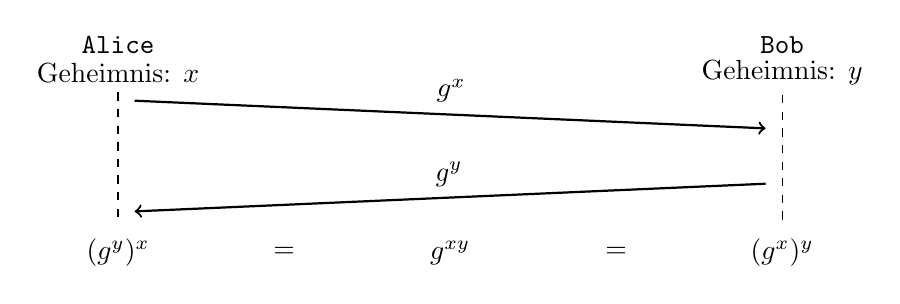
\begin{tikzpicture}[x=2em, y=2em]

      \draw (-6,0) node (Alice) {\texttt{Alice}};
      \draw (-6,-0.5) node (AliceSk) {Geheimnis: $x$};
      \draw (6,0) node (Bob) {\texttt{Bob}};
      \draw (6,-0.5) node (BobSk) {Geheimnis: $y$};
      
      % Lebenslinien
      \draw[dashed] (AliceSk) -- (-6,-3.25);
      \draw[dashed] (BobSk) -- (6,-3.25);
      
      % Pfeile fuer Nachrichten
      \textbf{\draw[->, thick] (-5.7,-1) -- (5.7,-1.5) node[sloped,above,pos=0.5] {$g^x$};}
      \textbf{\draw[->, thick] (5.7,-2.5) -- (-5.7,-3) node[sloped,above,pos=0.5] {$g^y$};}	
      
      % Beschriftung Ergebnis
      \draw (-6, -3.75) node {$(g^y)^x$};
      \draw (-3, -3.75) node {$=$};
      \draw (0, -3.75) node  {$g^{xy}$};
      \draw (3, -3.75) node  {$=$};
      \draw (6, -3.75) node  {$(g^x)^y$};

    \end{tikzpicture}
  \end{center}
  \caption{Diffie-Hellman-Schlüsselaustausch}
  \label{fig:keyex:dh}
\end{figure}
\subsubsection{Man-in-the-Middle-Angriff auf den
  Diffie-Hellman-Schlüsselaustausch}
Man-in-the-Middle-Angriffe sind eine häufige Art von Angriffen gegen
Netzwerkprotokolle. Hierbei versucht ein Angreifer, die Kommunikation
zwischen Alice und Bob dadurch zu übernehmen, dass er die ausgetauschten
Nachrichten abfängt und durch eigene ersetzt.

Im Fall des Diffie-Hellman-Schlüsselaustauschs kann ein Angreifer \A~,
der die Nachrichten manipulieren kann, den Schlüsselaustausch
kompromittieren. Dies wird in Abbildung \ref{fig:keyex:dh-angriff}
dargestellt. Der Angreifer wählt sich einen Zufallswert
$a$ und berechnet $g^a$. Das Ergebnis sendet er dann Alice und Bob, die
ihrerseits $g^x$ bzw. $g^y$ senden. Diese Nachrichten fängt \A~jedoch
ab, sodass Alice und Bob nie die Nachricht der jeweils anderen Partei
erhalten. Somit halten sie das $g^a$ für die Nachricht ihres
Gesprächspartners. Damit werden dann zwei Schlüssel $g^{xa}$ und
$g^{ya}$ erzeugt. Alice und Bob glauben, einen gemeinsamen Schlüssel
ausgetauscht zu haben. Sie haben aber jeweils einen gemeinsamen
Schlüssel mit \A~ausgetauscht.

Angenommen, Alice und Bob würden den Schlüssel nun für ein
Verschlüsselungsverfahren verwenden wollen. Verschlüsselt Alice nun eine
Nachricht, so tut sie dies mit dem Schlüssel $g^{xa}$. Sendet sie also ein
Chiffrat an Bob, so muss \A~dieses abfangen, entschlüsseln (\A~kennt
$g^{xa}$), mit $g^{ya}$ verschlüsseln und dann dieses Chiffrat an Bob
senden. Analog geht \A~vor, wenn Bob eine Nachricht an Alice
schickt. Damit lernt \A~alle Nachrichten, die Alice und Bob
austauschen. Zusätzlich muss \A~dies tun, um nicht aufzufallen. Würde
\A~eine Nachricht nicht so "neuverschlüsseln", so würde Bob bemerken,
dass er das Chiffrat nicht richtig entschlüsseln kann, womit der Angriff
auffällt.

Eine Lösung für dieses Problem ist, dass Alice und Bob ihre Nachrichten
signieren.
\begin{figure}[h]
  \begin{center}
    \scalebox{1}{
      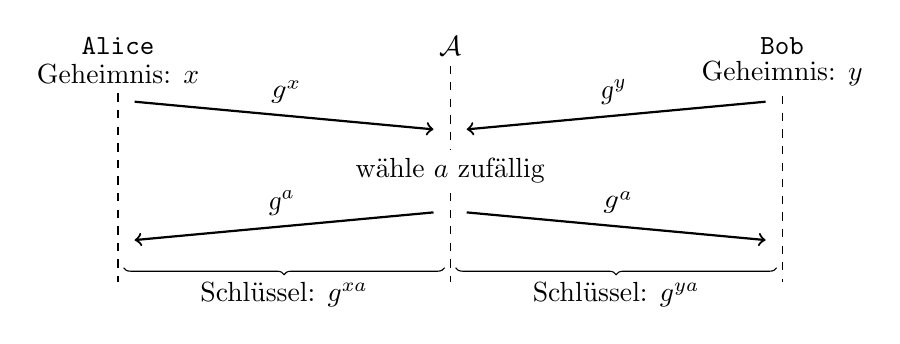
\begin{tikzpicture}[x=2em, y=2em]

        \draw (-6,0) node (Alice) {\texttt{Alice}};
        \draw (-6,-0.5) node (AliceSk) {Geheimnis: $x$};
        \draw (0,0) node (A) {$\mathcal{A}$};
        \draw (6,0) node (Bob) {\texttt{Bob}};
        \draw (6,-0.5) node (BobSk) {Geheimnis: $y$};
        
        \draw[dashed] (AliceSk) -- (-6,-4.25);
        \draw[dashed] (BobSk) -- (6,-4.25);
        
        
        \textbf{\draw[->, thick] (-5.7,-1) -- (-0.3,-1.5) node[sloped,above,pos=0.5] {$g^x$};}
        \textbf{\draw[->, thick] (5.7,-1) -- (0.3,-1.5) node[sloped,above,pos=0.5] {$g^y$};}	
        
        \draw (0,-2.25) node (ASk) {wähle $a$ zufällig};
        \draw[dashed] (A) -- (ASk);	
        \draw[dashed] (ASk) -- (0,-4.25);
        
        \textbf{\draw[->, thick] (-0.3,-3) -- (-5.7,-3.5) node[sloped,above,pos=0.5] {$g^a$};}
        \textbf{\draw[->, thick] (0.3,-3) -- (5.7,-3.5) node[sloped,above,pos=0.5] {$g^a$};}
        
        \draw[decorate, decoration={brace, mirror}] (-5.9,-4) -- node[below=0.4ex] {Schlüssel: $g^{xa}$} (-0.1,-4);
        \draw[decorate, decoration={brace, mirror}] (0.1,-4) -- node[below=0.4ex] {Schlüssel: $g^{ya}$} (5.9,-4);

      \end{tikzpicture}
    }
  \end{center}

  \caption{Man-in-the-Middle-Angriff auf Diffie-Hellman-Schlüsselaustausch}
  \label{fig:keyex:dh-angriff}    
\end{figure}
\section{Transport Layer Security (TLS)}\indexTLS
\label{sec:keyexchange:tls}
TLS (\emph{Transport Layer Security}) ist eine 1999 standardisierte
Weiterentwicklung des von Netscape entwickelten Protokolls SSL
(\emph{Secure Socket Layer}). Das Protokoll besteht aus 5
Teilprotokollen (siehe Tabelle \ref{tbl:tls}). Das Ziel von TLS ist es,
ein sicheres Verschlüsselungsverfahren für die Kommunikation über ein
unsicheres Netzwerk zu ermöglichen

\begin{table}[h]
\centering
\begin{tabular}{lllll}
\cline{1-4}
\multicolumn{1}{|c|}{\begin{tabular}[c]{@{}c@{}}TSL Handshake\\Protocol\end{tabular}} &
\multicolumn{1}{c|}{\begin{tabular}[c]{@{}c@{}}TSL Change Cipher Spec\\Protocol\end{tabular}} &
\multicolumn{1}{c|}{\begin{tabular}[c]{@{}c@{}}TSL Alert\\Protocol\end{tabular}} &
\multicolumn{1}{c|}{\begin{tabular}[c]{@{}c@{}}TSL Application Data\\Protocol\end{tabular}} & \\ \cline{1-4} \multicolumn{4}{|c|}{TLS Record
Protocol} & \\ \cline{1-4} & & & & \\ & & & &
\end{tabular}
\caption{Protokolle in TLS}
\label{tbl:tls}
\end{table}

TLS setzt auf die Transportschicht\indexTransportSchicht des OSI-Modell
auf\footnote{Die 
  Transportschicht ist die 4. Schicht des OSI-Modells, eine in Schichten
  gegliederte Architektur für Netzwerkprotokolle. Auf der 4. Schicht
  sind die bekannten Transportprotokolle TCP und UDP angesiedelt.}
. Dadurch kann TLS unabhängig von Anwendungen auf TCP aufgesetzt
werden. Den Teilprotokollen kommen dabei verschiedene Funktionen zu:
\begin{itemize}
\item Das \emph{TSL Handshake Protocol} initialisiert die
  Verschlüsselung. Dieses Protokoll führt den Schlüsselaustausch durch
  und wird im Folgenden näher betrachtet.
\item Das \emph{TLS Change Cipher Spec Protocol} enthält bloß ein Byte
  mit dem Inhalt \glqq 1\grqq. Dies dient dazu, die ausgehandelte
  Verschlüsselung zu aktivieren.
\item Das \emph{TSL Alert Protocol} meldet Fehler, die im Betrieb
  aufgetreten sind.
\item Das \emph{TSL Record Protocol} ist ein Dummy-Protokoll, dass die
  Daten der Anwendungen weiterreicht.
\item Das \emph{TLS Application Data Protocol} dient dazu, Daten mit den
  ausgehandelten Konfigurationen zu verschlüsseln.
\end{itemize}

\subsection{TLS-Handshake}\indexTLSHandshake 
Der Ablauf des TLS-Handshake-Protokolls ist in Abbildung
\ref{fig:keyex:tls-handshake} vereinfacht dargestellt.

Dafür signalisiert der Client dem Server, dass er den Aufbau eines
verschlüsselten Kanals wünscht (\emph{client\_hello}). Er liefert dem
Server eine Zufallszahl $R_C$ sowie eine nach seiner Präferenz sortierte
Liste von Algorithmen (Hashfunktionen, symmetrische
Verschlüsselungsverfahren und Schlüsselaustauschprotokolle). Der Server
generiert seinerseits eine Zufallszahl $R_S$, wählt einen Satz
Algorithmen aus der Liste des Clients aus und schickt diese zurück
(\emph{server\_hello}). Im Folgenden werden die vom Server ausgewählten
Verfahren verwendet.

Im nächsten Schritt schickt der Server dem Client ein Zertifikat, dass
seinen öffentlichen Schlüssel $pk_S$ enthält, damit der Client
die Identität seines Gesprächspartners überprüfen kann. Haben sich
Client und Server auf beidseitige Authentifikation geeinigt, fordert der
Server außerdem das Zertifikat des Clients an.  Wie genau diese
Authentifizierung abläuft, wurde im vorigen Schritt durch die Auswahl
der entsprechenden Algorithmen festgelegt. Der Client antwortet mit
seinem Zertifikat und seinem öffentlichen Schlüssel $pk_C$. Um die
Integrität der bisherigen Kommunikation sicherzustellen, berechnet der
Client außerdem den Hashwert $H$ der bisher ausgetauschten Nachrichten
und signiert diesen mit seinem privaten Schlüssel. Der Server prüft das
Zertifikat, die Signatur und den Hashwert.

Nun wählt der Client eine weitere Zufallszahl, das so genannte
\emph{premaster secret} (PMS)\indexTLSPreMasterSecret, und schickt es
verschlüsselt mit dem zertifizierten öffentlichen Schlüssel an den
Server. Beide Teilnehmer besitzen nun einen selbst gewählten Zufallswert
sowie einen des Kommunikationspartners und das premaster secret. Aus
diesen drei Zufallszahlen berechnen Client und Server nun mithilfe eines
öffentlich bekannten Algorithmus den \emph{master key}
(MS)\indexTLSMasterKey, aus dem wiederum die für die Kommunikation
verwendeten session keys abgeleitet werden.  Für die Berechnung der
jeweiligen Schlüssel werden Funktionen verwendet, die pseudozufällige
Ergebnisse liefern.

Im letzten Teil des Handshakes signalisiert der Client, dass er nun
verschlüsselt kommunizieren wird (\emph{ChangeCipherSpec}) und dass
damit der Handshake beendet ist (\emph{Finished}). Der Server antwortet
analog. Beide verwenden für die fortlaufende Kommunikation den
vereinbarten Verschlüsselungsalgorithmus und den gemeinsamen session
key.
\begin{figure}[h]
\begin{center}
\unitlength=1mm
\linethickness{0.4pt}
\hspace{-3 cm}
	\begin{picture}(120,150)(-10,0)
		\put(20,143){\makebox(0,0)[cb]{\texttt{Client}$_{\skey_C, \pkey_C}$}}
		\put(100,143){\makebox(0,0)[cb]{\texttt{Server}$_{\skey_S, \pkey_S}$}}
	
		\put(20,2){\line(0,1){140}}
		\put(100,2){\line(0,1){140}}
		
		\put(5,131){\makebox(0,0)[cb]{berechne}}
		\put(5,127){\makebox(0,0)[cb]{Zufallszahl $R_C$}}
		\put(60,123){\makebox(0,0)[cb]{\emph{client\_hello}(Liste$_{Algorithmen}$, $R_C$)}}
		\put(20,122){\vector(1,0){80}}
	
		\put(117,118){\makebox(0,0)[cb]{berechne}}
		\put(117,114){\makebox(0,0)[cb]{Zufallszahl $R_S$}}
		\put(60,110){\makebox(0,0)[cb]{\emph{server\_hello}(Auswahl$_{Algorithmen}$, $R_S$)}}
		\put(100,109){\vector(-1,0){80}}
		
		\put(60,100){\makebox(0,0)[cb]{Server-Zertifikat (inkl. $\pkey_S$)}}
		\put(100,99){\vector(-1,0){80}}
		\put(60,94){\makebox(0,0)[cb]{Anfrage Client-Zertifikat}}
		\put(100,93){\vector(-1,0){80}}
		
		\put(3,87){\makebox(0,0)[cb]{überprüfe}}
		\put(3,84){\makebox(0,0)[cb]{Server-Zertifikat}}
		
		\put(60,80){\makebox(0,0)[cb]{Client-Zertifikat (inkl. $\pkey_C$)}}
		\put(20,79){\vector(1,0){80}}
	
		\put(3,73){\makebox(0,0)[cb]{berechne Hash $H$}}
		\put(3,69){\makebox(0,0)[cb]{aller bisherigen}}
		\put(3,66){\makebox(0,0)[cb]{Nachrichten}}
		\put(60,62){\makebox(0,0)[cb]{$\sig(\skey_C, H)$}}
		\put(20,61){\vector(1,0){80}}
		
		\put(117,55){\makebox(0,0)[cb]{überprüfe $H$}}
		\put(117,51){\makebox(0,0)[cb]{und Signatur}}
		
		\put(3,55){\makebox(0,0)[cb]{berechne}}
		\put(3,51){\makebox(0,0)[cb]{Zufallszahl \emph{PMS}}}
		\put(60,47){\makebox(0,0)[cb]{$\enc(\pkey_S, \textit{PMS})$}}
		\put(20,46){\vector(1,0){80}}
		
		\put(3,40){\makebox(0,0)[cb]{berechne \emph{MS}}}
		\put(3,36){\makebox(0,0)[cb]{aus $R_C$, $R_S$, \emph{PMS}}}
		
		\put(117,40){\makebox(0,0)[cb]{berechne \emph{MS}}}
		\put(117,36){\makebox(0,0)[cb]{aus $R_C$, $R_S$, \emph{PMS}}}
		
		\put(60,32){\makebox(0,0)[cb]{\emph{ChangeCipherSpec}}}
		\put(20,31){\vector(1,0){80}}
		
		\put(60,26){\makebox(0,0)[cb]{\emph{Finished}}}
		\put(20,25){\vector(1,0){80}}
	
		\put(60,16){\makebox(0,0)[cb]{\emph{ChangeCipherSpec}}}
		\put(100,15){\vector(-1,0){80}}
		
		\put(60,10){\makebox(0,0)[cb]{\emph{Finished}}}
		\put(100,9){\vector(-1,0){80}}
	
	\end{picture}
\end{center}
\caption{Vereinfachter Ablauf eines SSL/TLS-Handshakes mit beidseitiger
  Authentifikation.} 
\label{fig:keyex:tls-handshake}
\end{figure}


\subsection{Angriffe auf TLS} Unter Verwendung einer idealen
Verschlüsselung, also im idealen Modell, ist TLS sicher. Auch in der
Praxis gilt die Sicherheit von TLS in der neuesten Version und
Verwendung der richtigen Parameter und Algorithmen als
ausreichend. Allerdings mussten konkrete Implementierungen als Reaktion
auf veröffentlichte Angriffe immer wieder gepatcht werden und es
existieren einige Angriffe auf bestimmte Varianten und Kombinationen von
eingesetzten Algorithmen, von denen im Folgenden einige erklärt werden.

\subsubsection{\texttt{ChangeCipherSpec} Drop} Dieser Angriff entstammt
dem Jahr 1996 und richtet sich gegen SSL unter Version 3.0, also gegen
das Protokoll \emph{vor} seiner Standardisierung als TLS.
\begin{description}
\item[Beobachtung:] Server und Client tauschen zu Beginn ihrer
  Kommunikation eine Reihe unverschlüsselter Nachrichten aus (öffentliche
  Schlüssel, Präferenzen für verwendete Algorithmen, Details der
  Authentifikation \ldots), die es einem Angreifer erlauben, den Status
  des Schlüsselaustauschs zu erkennen. Kurz vor Ende des Handshakes sendet
  der Client, ebenfalls im Klartext, \emph{ChangeCipherSpec}, um auf
  verschlüsselte Kommunikation umzuschalten.
\item[Angriff:] Ein aktiver Angreifer unterdrückt den
  \emph{ChangeCipherSpec}-Hinweis des Clients.
\item[Konsequenz:] Falls der Server sofort danach Nutzdaten
  sendet, werden diese nicht verschlüsselt und können vom Angreifer von
  der Leitung gelesen werden.
\item[Gegenmaßnahme:] Bevor die Nutzdaten gesendet werden, muss
  der Server auf die Bestätigung des Clients warten.
\end{description}

\subsubsection{Beispielangriff auf RSA-Padding} 1998 wurde ein Angriff
auf das RSA-Padding bekannt, der bei entsprechender Algorithmenwahl in
SSL ausgenutzt werden kann, um Einblick in den für die gemeinsame
Kommunikation verwendeten Schlüssel zu erlangen.
\begin{description}
\item[Beobachtung:] Die von SSL eingesetzte Variante von RSA
  verwendet beim Transport des Master Keys\indexTLSMasterKey "`naives"'
  Padding:
  \begin{align*} C = \enc(\pkey, \text{pad}(M)) =
    (\text{pad}(M))^e \mod N
  \end{align*} Dabei kann durch homomorphe Veränderungen
  des Chiffrats $C$ und ständige Überprüfung, ob $C$ noch immer gültig
  ist, auf die Beschaffenheit von $M$ geschlossen werden.
\item[Angriff:] Eine vereinfachte Darstellung des zu
  übertragenden Schlüssels $K$ ist:
  \begin{align*} C = \text{pad}(K)^e =
    (0\mathrm{x}0002 \parallel \mathtt{rnd} \parallel
    0\mathrm{x}00 \parallel K)^e \mod N
  \end{align*} Klar ist, dass $K$ vergleichsweise kurz
  sein und deshalb mit vielen Nullbits beginnen muss. Ziel ist es nun,
  möglichst viele gültige Faktoren $\alpha_i$ zu finden, sodass
  \begin{align*} M_i \coloneqq \alpha_i \cdot
    (0\mathrm{x}0002 \parallel \mathtt{rnd} \parallel
    0\mathrm{x}00 \parallel K) \mod N = \dec(\alpha_i^e \cdot C \mod N)
  \end{align*} gültig ist. Die Gültigkeit wird
  festgestellt, indem die $M_i$ zur Überprüfung an den Server
  weitergeleitet werden. Der Server gibt in älteren SSL-Versionen
  Hinweise, wenn das Padding fehlerhaft ist.
\item[Konsequenz:] Viele gültige $M_i$ liefern ein grobes
  Intervall, in dem $K$ liegt.
\item[Gegenmaßnahme:] Wähle $K$ zufällig, wenn das Padding
  ungültig ist. (Zu diesem Zeitpunkt stand eigentlich bereits RSA-OAEP zur
  Verfügung.)
\end{description} 
Aus diesem Angriff geht das Theorem von Håstad und Näslund hervor, das
besagt, dass jedes Bit von RSA \emph{hardcore} ist.
\begin{theorem}[Håstad und Näslund] Sei N, e, d wie bei RSA, $M^* \in
\mathbbm{Z}_N$ und $i \in \{1, \ldots , \lfloor \log_2(N)\rfloor \}$
beliebig. Sei $\mathcal{O}$ ein Orakel, das bei Eingabe $C$ das i-te Bit
von $M = C^d \mod N$ ausgibt. Dann existiert ein (von N, e, d
unabhängiger) Polynomialzeit-Algorithmus, der bei Eingabe N, e, i und
$C^* \coloneqq (M^*)^e \mod N$ und mit $\mathcal{O}$-Zugriff $M^*$ berechnet.
\end{theorem}

\subsubsection{CRIME}
\label{sec:keyex:crime}
Dieser Angriff aus 2002 (Aktualisierung in 2012) funktioniert bei
eingeschalteter Kompression. 
\begin{description}
\item[Beobachtung:] Bei eingeschalteter Kompression wird nicht mehr $M$
  sondern \emph{comp}$(M)$ übertragen. TLS verwendet
  \emph{DEFLATE}-Kompression. Bereits einmal aufgetretene Muster werden
  also nach dem Prinzip \emph{comp}\texttt{(Fliegen fliegen) = Fliegen
    f(-8,6)} wiederverwendet.
\item[Angriff:] Ein Angreifer kann über die Länge des Chiffrats
  feststellen, ob im nachfolgenden (unbekannten) Teil des Klartextes
  Kompression verwendet wurde, indem er einen vorangegangenen Teil
  manipuliert. Die Länge des Chiffrats sinkt dann und der Angreifer weiß,
  dass zumindest ein Teil seines selbst eingefügten Textes im Rest des
  Chiffrats vorgekommen sein muss.
  
  Konkret kann sich ein Angreifer, der in der Lage ist, einem Client
  einen Teil seiner Kommunikation mit dem Server zu diktieren, Stück für
  Stück dem von ihm gesuchten Klartext nähern. Wenn er beispielsweise den
  Session-Cookie des Clients (mit dem geheimen Inhalt \texttt{ABCD})
  stehlen möchte, so kann er (z.B. über Schadcode) dem Client eine Eingabe
  (z.B. \texttt{WXYZ}) diktieren, die dieser vor dem Verschlüsseln der
  Nachricht hinzufügt. Er komprimiert und verschlüsselt also nicht mehr
  nur \texttt{ABCD} sondern \texttt{WXYZABCD}. Aus dem belauschten
  Chiffrat $C \coloneqq \enc(K, \mathit{comp}(\mathtt{WXYZABCD}))$ kann der
  Angreifer die Länge von $\mathit{comp}(\mathtt{WXYZABCD})$ extrahieren
  und so den Abstand seines eingeschleusten Textstücks \texttt{WXYZ} zu
  dem vom Client geheim gehaltenen Cookie bestimmen.
\item[Konsequenz:] Mit mehreren Wiederholungen kann der Angreifer den
  Inhalt des Cookies immer weiter einschränken und ihn schließlich
  rekonstruieren.
\item[Gegenmaßnahme:] Keine Kompression verwenden.
\end{description}

\subsubsection{Logjam}
Logjam\cite{Adrian2015} ist ein 2015 veröffentlichter Angriff auf das
TLS-Handshake-Protokol. Es ermöglicht einem Man-in-the-Middle-Angreifer
den Server zur Verwendung eines unsicheren Verfahrens zu bringen.
\begin{description}
\item[Beobachtung:] 
  Die ersten Nachrichten des Handshakes sind nicht verschlüsselt. Die
  Absicherung der Integrität wird erst über die Signatur nach dem
  Austausch der Zertifikate erreicht.
\item[Angriff:] Der Angreifer fängt die \emph{client\_hello}-Nachricht ab
  und ersetzt die Liste der Schlüsselaustausch-Verfahren durch eine
  Liste, die lediglich Diffie-Hellman-Schlüsselaustausch mit Schlüsseln
  von 512-bit Länge enthält. Diese manipulierte Nachricht sendet er an
  den Server weiter. Dieser wählt dann das schwache Verfahren aus.
  Der Angreifer hat jetzt bis zum Senden der Signatur über die Hashes
  der bisher gesendeten Nachrichten Zeit, das Verfahren zu brechen und
  an den geheimen Schlüssel zu kommen. Dies braucht zwar einige
  Vorberechnungen, ist aber trotzdem praktikabel.
\item[Konsequenz:] Der Angreifer kann sich als
  Man-in-the-Middle-Angreifer in die verschlüsselte Kommunikation
  einklinken und Nachrichten beliebig manipulieren.
\item[Gegenmaßnahme:] Der Server darf schwache Verschlüsselungen nicht
  akzeptieren, sondern muss den Aufbau von Verbindungen zurückweisen,
  wenn er vom Client lediglich schwache Verfahren vorgeschlagen bekommt.
\end{description}

\subsubsection{Fazit}
TLS\indexTLS ist ein historisch gewachsenes Protokoll mit hoher
Relevanz. Allerdings bietet es durch die hohe Anzahl an Versionen und
Einstellungsmöglichkeiten auch eine große Angriffsfläche, die häufiger
durch Fixes als durch Einführung sichererer Algorithmen reduziert
wird. Dazu kommt, dass von vielen Browsern ausschließlich der
TLS-Standard von 1999 unterstützt wird, was zwar Schwierigkeiten in der
Kompatibilität mit anderen Systemen umgeht, aber auch dazu führt, dass
einige bereits bekannte Ansatzpunkte für Angriffe noch immer
flächendeckend bestehen.

\section{Weitere Protokolle}

\subsection{IPsec}\indexIPsec
IPsec (\emph{Internet Protocol Security}) ist eine Sammlung von
Standards, die zur Absicherung eines IP-Netzwerks entworfen wurden. Es
setzt demnach nicht wie TLS auf der Transportschicht sondern auf der
Internetschicht des TCP/IP-Protokollstapels auf. Es soll die Schutzziele
Vertraulichkeit, Integrität und Authentizität in IP-Netzwerken
sicherstellen. Allerdings liegt der Fokus von IPsec dabei nicht auf dem
Schlüsselaustausch, der deshalb vorher getrennt stattfinden muss
(aktuell durch IKE). Stattdessen bietet IPsec Maßnahmen zur
Integritätssicherung der Daten an (u.A. HMAC), soll die Vortäuschung
falscher IP-Adressen (IP-Spoofing) verhindern und bietet verschiedene
Modi zur Verschlüsselung von IP-Paketen an.

Obwohl IPsec nicht sonderlich stark verbreitet und nicht sehr gut
untersucht ist, haben sich bereits einige Angriffe herauskristallisiert,
auf die hier jedoch nicht näher eingegangen wird.


\subsection{Password Authentication Key Exchange (PAKE)}\indexPAKE
Dieses Protokoll basiert auf der Annahme, dass Alice und Bob, die
miteinander kommunizieren wollen, ein gemeinsames Geheimnis
\texttt{passwort} besitzen. Über dieses Passwort wollen sie einander
authentifizieren und einen Schlüssel für ihre Kommunikation
errechnen. Natürlich kann ein Angreifer trotz allem noch eine
vollständige Suche über die möglichen Passwörter durchführen, es sollte
ihm jedoch nicht möglich sein, schneller ans Ziel zu kommen.

Es handelt sich dabei eher um ein grundlegendes Prinzip als um ein
feststehendes Protokoll. Bei der Konstruktion eines PAKE ist darauf zu
achten, dass die simpelste Variante, das Senden von
$\enc(\mathtt{passwort}, \key)$ keine forward-secrecy bietet. Das
bedeutet, wenn im Nachhinein ein Angreifer das Passwort eines
Teilnehmers knackt, ist er nicht nur zukünftig in der Lage, dessen
Identität zu simulieren sondern kann außerdem sämtliche vergangene
Kommunikation nachvollziehen.

Eine funktionierende Konstruktion ist \emph{Encrypted Key Exchange}
(EKE), bei dem zunächst $\enc(\mathtt{passwort},\pkey)$ gesendet und
infolgedessen asymmetrisch kommuniziert wird. Bei \emph{Simple Password
Exponential Key Exchange} wird ein Diffie-Hellman-Schlüsselaustausch auf
der Basis von einem nur den Teilnehmern bekannten $g =
H(\mathtt{passwort})^2$ durchgeführt. Der beweisbare PAKE von
Goldreich-Lindell nutzt Zero-Knowledge, um die Teilnehmer zu
authentifizieren, ohne das dafür nötige Geheimnis aufzudecken.

PAKE wird z.B. als Basis für EAP (\emph{Extensible Authentication
Protocol}) in WPA verwendet und ist formal modellierbar und seine
Sicherheit unter bestimmten theoretischen Annahmen beweisbar.

%%% Local Variables:
%%% mode: latex
%%% TeX-master: "skript"
%%% End:
